%==============================================================================
\section{Combining PINGU with JUNO}
\label{sec:JUNO}
%==============================================================================


\subsection{The JUNO Experiment}
\label{sec:JUNO_exp}

\begin{figure}[thp]
 \centering
 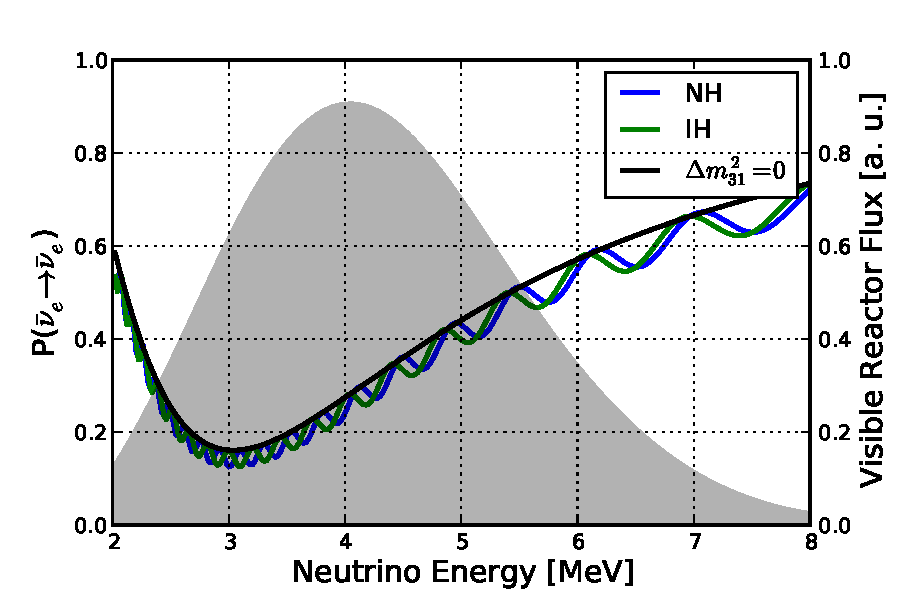
\includegraphics[width=0.7\linewidth]{JUNO_osc_probs}
 \caption{\nuebar survival probability for a baseline of 50\,km, overlaid with
  the un-oscillated nuclear reactor spectrum as it would be detected by JUNO
  (including detector acceptance).}
 \label{fig:JUNO_osc_probs}
\end{figure}

As already briefly discussed in Sec.~\ref{sec:ReacNuOsc}, JUNO\footnote{Short
for Jiangmen Underground Neutrino Observatory.} is a neutrino experiment under
construction in China's Guangdong Province. With its sensitive region at low MeV
energies, it is able to detect supernova and geoneutrinos, yet its main target
are reactor neutrinos from the Taishan and Yangjiang nuclear power plants to be
erected in $\approx 50$\,km distance each. These \nuebar's can be detected via
inverse beta decay:
\begin{equation}
 ^A_Z\mathrm{X} + \nuebar \quad \to\quad  ^A_{Z-1}\mathrm{Y} + e^+
\end{equation}

These \nuebar undergo oscillations that are mostly due to the smaller mass
splitting \dm{21}, but have a fast modulation due to \dm{31}. The vacuum \nuebar
survival probability\footnote{Matter effects can be neglected here.} can be
expressed analytically:
\begin{eqnarray}
 P(\nuebar\to\nuebar)\quad = \quad 1 &-& \cos^4(\thet{13})\,\sin^2(2\thet{12})\,
                            \sin^2\left(\dm{21}\frac{L}{4E}\right) \nonumber\\
                          &-& \cos^2(\thet{12})\, \sin^2(2\thet{13})\,
                            \sin^2\left(\dm{31}\frac{L}{4E}\right) \nonumber\\
                          &-& \sin^2(\thet{12})\, \sin^2(2\thet{13})\,
                            \sin^2\left(\dm{32}\frac{L}{4E}\right)
 \label{eqn:JUNO_osc_probs}
\end{eqnarray}
with $\dm{32} = \dm{31} - \dm{21}$. As shown in Fig.~\ref{fig:JUNO_osc_probs},
for a baseline of $L = 50$\,km this is dominated by the slow \dm{21}
oscillation, corresponding to the first term in (\ref{eqn:JUNO_osc_probs}). On
top of that is a pattern of rapid oscillation originating from the interference
of the second and third term of (\ref{eqn:JUNO_osc_probs}). The exact shape of
this pattern, especially the position of the local minima and maxima, depend on
the mass hierarchy which changes the relative sizes of \dm{31} and
\dm{32}\footnote{Their signs are irrelevant as the outer $\sin^2$ is symmetric
about zero.}.

\begin{figure}[thp]
 \centering
 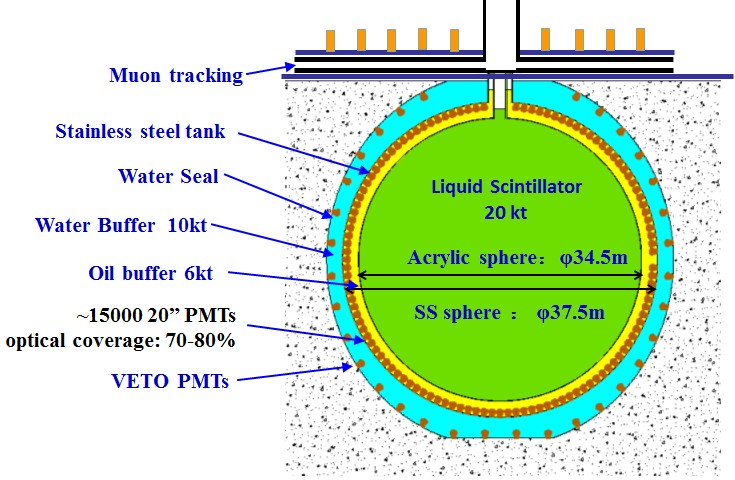
\includegraphics[width=0.7\linewidth]{JUNO}
 \caption{Layout of the JUNO detector. Figure taken from \cite{JUNO2}.}
 \label{fig:JUNO_layout}
\end{figure}

Taking the detector acceptance into account, the expected reactor neutrino
spectrum \cite{JUNO_TDR} is very suitable to observe this signal, as one can see
in Fig.~\ref{fig:JUNO_osc_probs} as well. However, a very precise energy
reconstruction is needed to actually resolve the spectral features associated
with the neutrino mass hierarchy.

With the detector setup shown in Fig.~\ref{fig:JUNO_layout}, a relative
resolution of $3\,\%/\sqrt{E [\mathrm{MeV}]}$ is aimed for. The target volume
is filled with 20\,kt of liquid scintillator to enhance the photon output. This
essentially destroys any directionality of the event signatures, however, no
information about the arrival direction of the neutrinos is needed as the
baseline for the oscillation is known\footnote{In PINGU, the \coszen
information is needed to infer the location where the neutrinos were generated
in the Earth's atmosphere and hence the distance they have travelled.}. The
inner surface of the volume is covered with $\approx 15000$ 20'' PMTs, resulting
in a photocoverage of at least 70\,\%. Tagging and vetoing of atmospheric muons
is ensured by scintillator tiles on top of the detector and a 10\,kt water
Cherenkov detector surrounding the target volume. Natural radioactivity is
buffered in a layer between muon veto and active region filled with 6\,kt of
mineral oil \cite{JUNO2}.

If this precision can indeed be realised, JUNO claims to be able to determine
the neutrino mass hierarchy with a significance of $\approx 3.3\,\sigma$ with a
total $10^5$ recorded neutrino events, corresponding to six years of data taking
\cite{JUNO, JUNO2, JUNO_TDR}. In the following sections a modification of \papa
is described, aiming at a detector simulation for JUNO instead of PINGU in order
to reproduce the reported sensitivity.

\subsection{Simulating JUNO with \papa}
\label{sec:JUNO_sim}

The major difference between the observable signals in PINGU and JUNO is that
PINGU will record a two-dimensional histogram in ($E$,\,\coszen) while in JUNO
only the energy spectrum is measured. Thus only one very narrow zenith bin
with edges at $\coszen = [-0.0039245,\,-0.0039235]$ is simulated, corresponding
to a baseline of 50\,km. In energy, 300 bins between 2\,MeV and 8\,MeV are
used. No oversampling is applied as the oscillation probabilities are
already sufficiently smooth (see Fig.~\ref{fig:JUNO_osc_probs}).

Since only the \nuebar survival probability is relevant for JUNO, which can be
calculated analytically according to (\ref{eqn:JUNO_osc_probs}), the
\texttt{PhysicsSimulation} has been extended by a module doing exactly this
analytical calculation. Avoiding the numerical solution of the Schr\"{o}dinger
equation, the \texttt{PhysicsSimulation} is sped up dramatically.

For the \texttt{DetectorSimulation}, the software itself is not changed,
however the inputs of course have to model the JUNO detector.
The neutrino flux is adopted from \cite{JUNO_TDR} and stored in a table of the
same format as the atmospheric flux tables provided by \cite{HondaSP}. This
flux, shown as an overlay in Fig.~\ref{fig:JUNO_osc_probs}, has the detector
acceptance already folded in, but is only given in arbitrary units. Thus, the
effective area is set to a constant value of 1\,m$^2$ for \nuebar CC and zero
for all other interaction channels while the analysis histograms will be
normalised to $10^5$ \nuebar events before analysis.

The directional reconstruction is parametrised by a single Gaussian with a
fixed width of $10^{-5}$ in \coszen, meaning that all events will stay in
place. As there is only one bin in \coszen, migration of events is impossible
in any case.

The energy reconstruction is represented by a single Gaussian as well, with
mean and width given by
\begin{eqnarray}
 \mu(E) &=& E - 0.8\,\mathrm{MeV} \\
 \sigma(E)/E &=& 4\,\%/\sqrt{E [\mathrm{MeV}] - 0.8} \quad.
\end{eqnarray}
The shift in energy reflects the fact that the visible energy in an inverse beta
decay is smaller than the initial neutrino energy. 511\,keV are needed to
create the $e^+$, which in turn stops to emit Cherenkov light once it falls
below the Cherenkov threshold (\ref{eqn:ChkovThr}), corresponding to a kinetic
energy of $\approx 280$\,keV depending on the optical medium. These two
contributions sum up to $\approx 0.8$\,MeV.
The relative energy resolution refers to the visible energy as well.
Additionally, it has been deteriorated \wrt the published specifications to be
$4\,\%/\sqrt{E_\mathrm{vis} [\mathrm{MeV}]}$. This reflects the fact that the
nuclear power plants used as neutrino sources have several reactor cores that
are up to 500\,m apart from each other. This introduces an uncertainty of 1\,\%
on the baseline $L$, which is equivalent to an additional uncertainty of 1\,\%
in the energy reconstruction as the relevant quantity is $L/E$.

\subsection{Joint Analysis of JUNO and PINGU}
\label{sec:JUNO_comb}